\documentclass[conference]{IEEEtran}

\usepackage[T1]{fontenc}
\usepackage[utf8]{inputenc}
\usepackage[brazil]{babel}
\usepackage{amsmath}
\usepackage{graphicx}
\usepackage{booktabs}
\usepackage{cite}
\usepackage{url}
\usepackage{microtype}
\usepackage{float}

\graphicspath{{imagens/}}

\title{Classificação do Dataset Iris com PCA e K-NN}

\author{
\IEEEauthorblockN{Felipe Duarte Silva \quad Paulo Henrique Jankosz}
\IEEEauthorblockA{
GRR20231957 \quad GRR20220627\\
Departamento de Informática -- UFPR}
}

\begin{document}
\maketitle

\begin{abstract}
Este trabalho analisa o dataset Iris (150 amostras, 3 espécies, 4
variáveis morfológicas) por meio de estatísticas descritivas, análise de
correlação, PCA e classificação K-NN. A PCA com dois componentes
preserva 95,8\% da variância. O K-NN com $K=1$ atingiu 96,67\% de
acurácia no teste, errando uma única amostra.
\end{abstract}

\section{Introdução}

O dataset Iris, publicado por Fisher~\cite{fisher1936}, contém 150
amostras de três espécies (\textit{Iris-setosa}, \textit{Versicolor} e
\textit{Virginica}), com 50 observações cada. As quatro variáveis são
comprimento e largura da sépala e da pétala, em centímetros. O conjunto
foi obtido do UCI Machine Learning Repository~\cite{uci_iris} e não
possui valores ausentes.

O objetivo é explorar a estrutura dos dados e classificar as espécies.
A implementação usa Python com scikit-learn, pandas e
matplotlib.

\section{Análise Exploratória}

\subsection{Estatísticas descritivas}

A Tabela~\ref{tab:stats} resume média, desvio e moda de cada variável,
tanto no geral quanto por espécie. As variáveis de pétala apresentam
desvio-padrão bem maior (1,76 e 0,76) que as de sépala (0,83 e 0,43),
indicando maior dispersão e potencial discriminativo. A Setosa se
destaca por pétalas muito pequenas (média 1,46~cm de comprimento),
enquanto a Virginica tem os maiores valores em quase todas as medidas.

\begin{table}[H]
\centering
\caption{Média / desvio / moda por variável e classe.}
\label{tab:stats}
\setlength{\tabcolsep}{3pt}
\footnotesize
\begin{tabular}{lccccccccc}
\toprule
 & \multicolumn{3}{c}{Geral} & \multicolumn{2}{c}{Setosa} &
   \multicolumn{2}{c}{Versic.} & \multicolumn{2}{c}{Virgin.} \\
\cmidrule(lr){2-4}\cmidrule(lr){5-6}\cmidrule(lr){7-8}\cmidrule(lr){9-10}
Variável & $\mu$ & $\sigma$ & moda & $\mu$ & $\sigma$ & $\mu$ & $\sigma$ & $\mu$ & $\sigma$ \\
\midrule
C.\ sép. & 5,84 & 0,83 & 5,0 & 5,01 & 0,35 & 5,94 & 0,52 & 6,59 & 0,64 \\
L.\ sép. & 3,05 & 0,43 & 3,0 & 3,42 & 0,38 & 2,77 & 0,31 & 2,97 & 0,32 \\
C.\ pét. & 3,76 & 1,76 & 1,5 & 1,46 & 0,17 & 4,26 & 0,47 & 5,55 & 0,55 \\
L.\ pét. & 1,20 & 0,76 & 0,2 & 0,24 & 0,11 & 1,33 & 0,20 & 2,03 & 0,27 \\
\bottomrule
\end{tabular}
\end{table}

\subsection{Relação entre variáveis}

No espaço da sépala as três classes se sobrepõem bastante, com
correlação de Pearson geral de $r = -0{,}11$, embora dentro de cada
classe a correlação seja positiva (Setosa: 0,75; Versicolor: 0,53;
Virginica: 0,46). Essa inversão é um exemplo do Paradoxo de Simpson.

Já no espaço da pétala (Figura~\ref{fig:petala}) a separação é muito
mais nítida: a Setosa forma um agrupamento isolado, e Versicolor e
Virginica se distribuem com sobreposição apenas na fronteira. A
correlação geral sobe para $r = 0{,}96$.

\begin{figure}[H]
    \centering
    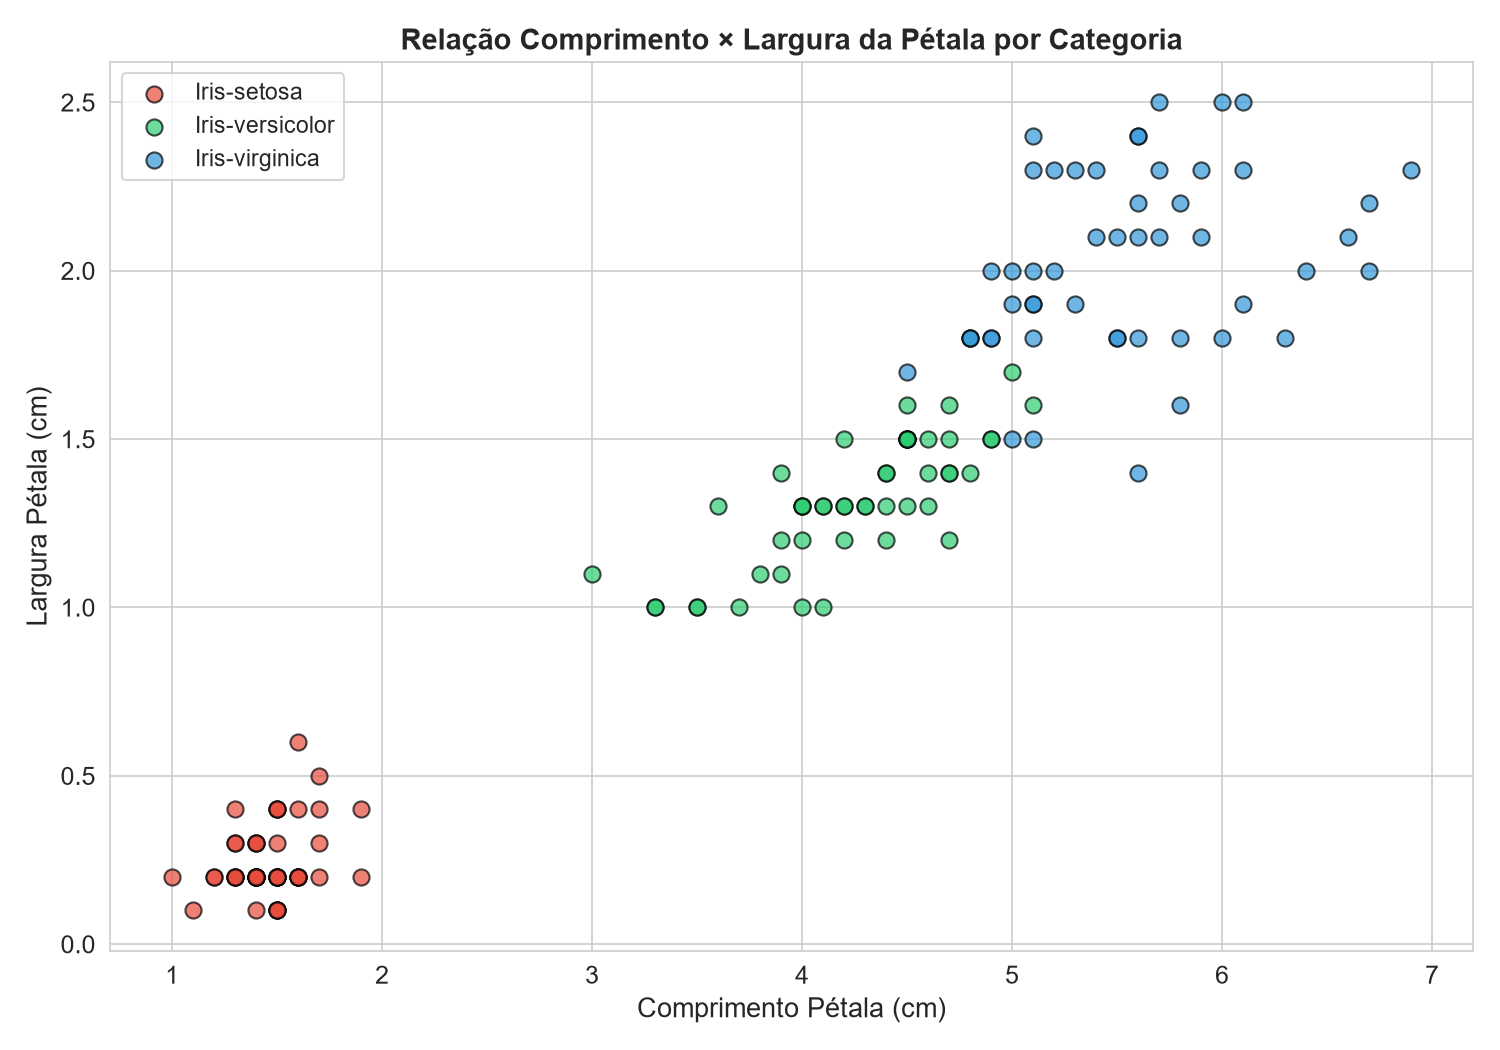
\includegraphics[width=0.88\columnwidth]{03_petala_comprimento_largura.png}
    \caption{Comprimento $\times$ largura da pétala por espécie.}
    \label{fig:petala}
\end{figure}

Histogramas e boxplots das quatro variáveis confirmam que as dimensões
de pétala oferecem a melhor discriminação entre as espécies, enquanto as
de sépala possuem distribuições muito sobrepostas.

\section{PCA}

A PCA~\cite{jolliffe2016} foi aplicada sobre os dados padronizados
(média zero, variância unitária). A Tabela~\ref{tab:pca} mostra que os
dois primeiros componentes concentram 95,8\% da variância, permitindo
uma boa representação 2D. O PC1 (72,8\%) é dominado pelas medidas de
pétala e pelo comprimento da sépala, enquanto o PC2 (23,0\%) depende
principalmente da largura da sépala.

\begin{table}[H]
\centering
\caption{Variância explicada por componente principal.}
\label{tab:pca}
\begin{tabular}{lcc}
\toprule
Comp. & Variância (\%) & Acumulada (\%) \\
\midrule
PC1 & 72,77 & 72,77 \\
PC2 & 23,03 & 95,80 \\
PC3 &  3,68 & 99,48 \\
PC4 &  0,52 & 100,00 \\
\bottomrule
\end{tabular}
\end{table}

A Figura~\ref{fig:pca} mostra a projeção 2D. A Setosa fica
completamente separada à esquerda, enquanto Versicolor e Virginica se
distinguem ao longo do PC1 com pequena sobreposição na região central.

\begin{figure}[H]
    \centering
    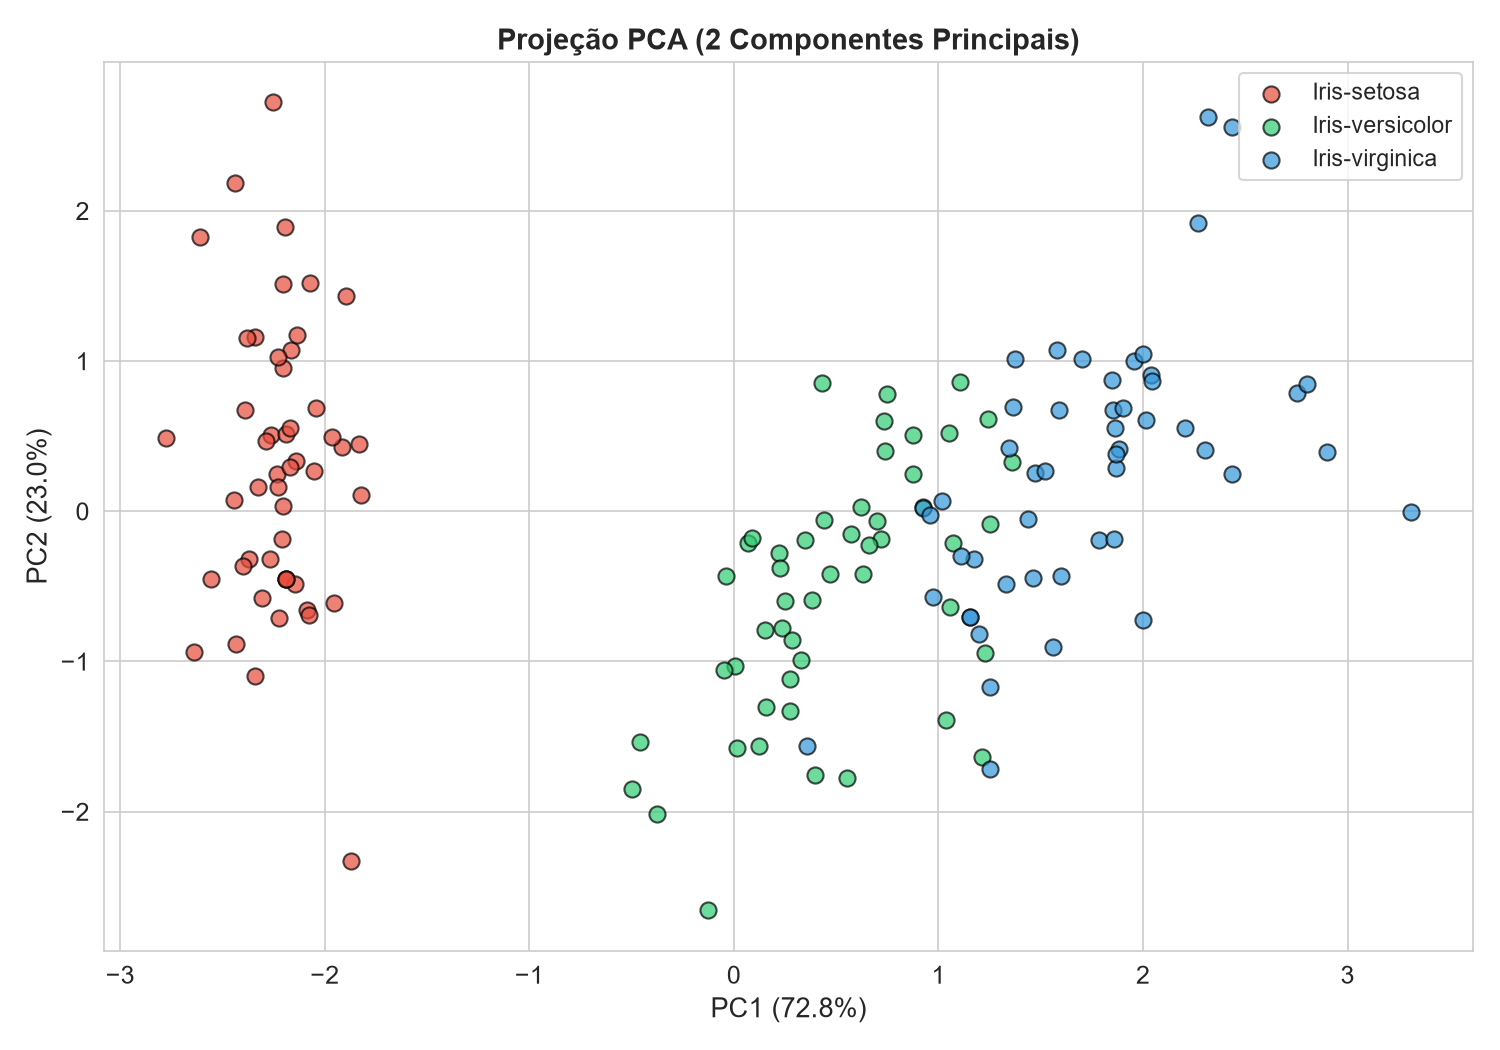
\includegraphics[width=0.88\columnwidth]{08_pca_projecao_2d.png}
    \caption{Projeção PCA em 2 componentes (95,8\% da variância).}
    \label{fig:pca}
\end{figure}

\section{Classificação com K-NN}

O dataset foi dividido em 80\% treino (120 amostras) e 20\% teste (30
amostras), com estratificação. Os dados foram padronizados, o que é
importante para o K-NN por ele usar distância euclidiana~\cite{cover1967}.
Testamos $K$ de 1 a 20 e o melhor resultado veio com $K = 1$, alcançando
acurácia de 96,67\% (29/30 acertos). A Tabela~\ref{tab:knn} detalha as
métricas.

\begin{table}[H]
\centering
\caption{Métricas do K-NN ($K=1$).}
\label{tab:knn}
\begin{tabular}{lcccc}
\toprule
Classe & Prec. & Recall & F1 & Sup. \\
\midrule
Setosa      & 1,00 & 1,00 & 1,00 & 10 \\
Versicolor  & 0,91 & 1,00 & 0,95 & 10 \\
Virginica   & 1,00 & 0,90 & 0,95 & 10 \\
\midrule
Acurácia    & \multicolumn{4}{c}{96,67\%} \\
\bottomrule
\end{tabular}
\end{table}

A Setosa foi classificada sem nenhum erro. O único equívoco foi uma
Virginica rotulada como Versicolor, na fronteira entre as duas classes.
A Figura~\ref{fig:cm} traz a matriz de confusão correspondente.

\begin{figure}[H]
    \centering
    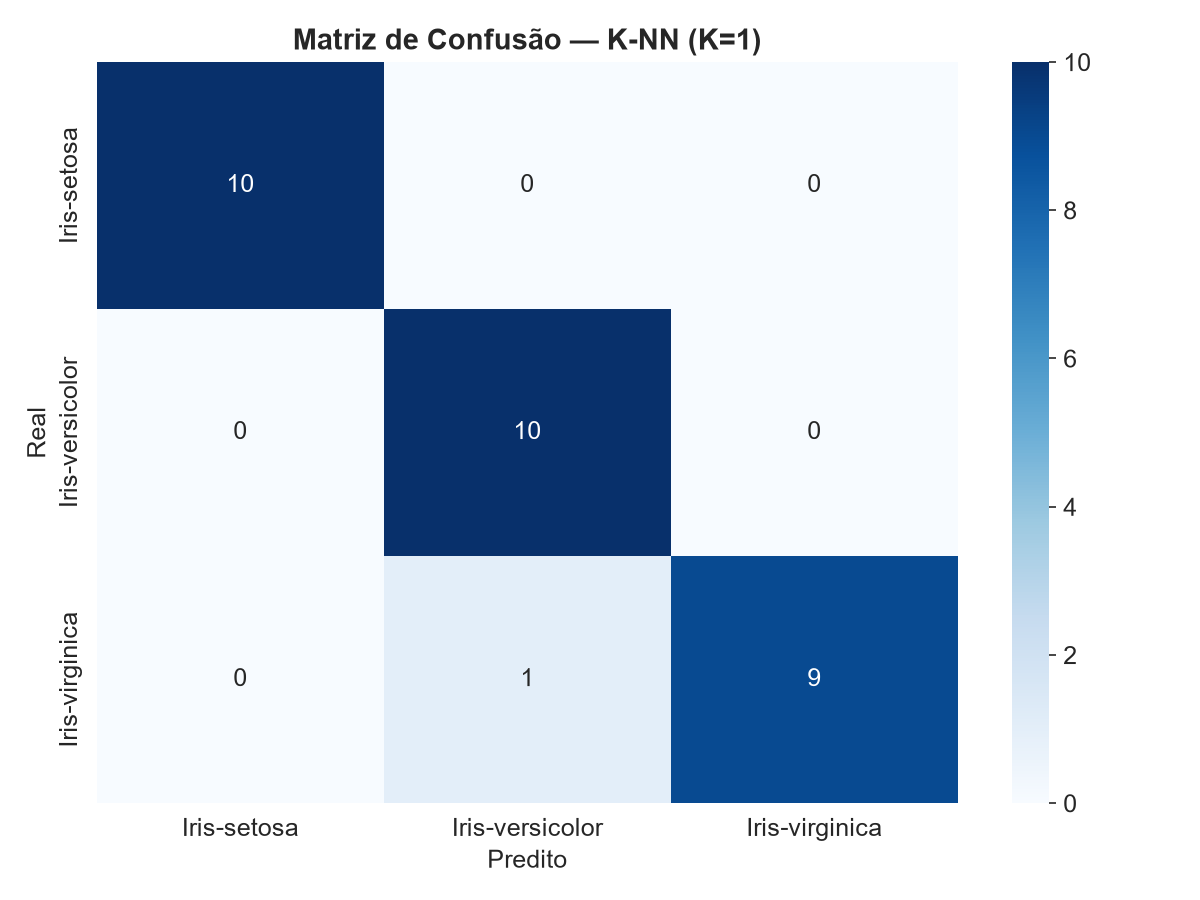
\includegraphics[width=0.75\columnwidth]{11_knn_matriz_confusao.png}
    \caption{Matriz de confusão do K-NN ($K=1$).}
    \label{fig:cm}
\end{figure}

\section{Conclusão}

As medidas de pétala são as mais úteis para separar as três espécies,
isolando completamente a Setosa. A PCA com dois componentes preserva
95,8\% da informação, e o K-NN com $K=1$ alcança 96,67\% de acurácia. O
único erro ocorre justamente onde Versicolor e Virginica se sobrepõem,
resultado coerente com tudo que foi observado na análise exploratória.

\begin{thebibliography}{00}

\bibitem{fisher1936}
R.~A.~Fisher, ``The use of multiple measurements in taxonomic
problems,'' \emph{Annals of Eugenics}, vol.~7, no.~2, pp.~179--188,
1936.

\bibitem{uci_iris}
D.~Dua e C.~Graff, ``UCI Machine Learning Repository,'' 2019.
[Online]. Available:
\url{https://archive.ics.uci.edu/ml/datasets/iris}.

\bibitem{jolliffe2016}
I.~T.~Jolliffe e J.~Cadima, ``Principal component analysis: a review
and recent developments,'' \emph{Phil.\ Trans.\ Royal Soc.\ A},
vol.~374, no.~2065, 2016.

\bibitem{cover1967}
T.~Cover e P.~Hart, ``Nearest neighbor pattern classification,''
\emph{IEEE Trans.\ Inf.\ Theory}, vol.~13, no.~1, pp.~21--27, 1967.

\end{thebibliography}

\end{document}
